\chapter{Analyses Methodology}
\label{chap:estimation}
In this section, an overview of the procedure to calculate the fatigue life is presented. Figure \ref{fig:aanaalg} illustrates the analysis algorithm. 
\begin{figure}[H]
\centering
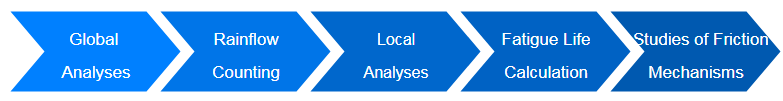
\includegraphics[scale=0.73]{figures/anaaalg}
\caption[Algorithm for calculation of fatigue life ]{Algorithm for calculation of fatigue life  }
 \label{fig:aanaalg}
\end{figure}
\section{Global Analysis}
The global analyses were performed by exposing the global model in far configuration to all 160 sea states in Figure \ref{fig:scatn} with one-hour record length. The following three resulting quantities from the analyses were stored in separate files for each time step and each sea state:
\begin{itemize}
    \item The tension in the upper element of the cable.
    \item The displacement of the dummy node on the vessel in x-, y-, and z-direction.
    \item The displacement of the supernode at the cable hang off, and subsequent node in the top the cable in x-, y- and z-direction.
\end{itemize}

\subsection{Post Processing of Global Analyses Results}
The angle ($\theta$) between the vessel and cable in Figure \ref{fig:angle} was calculated and turned into time series by dot product as in Equation \ref{eq:dot}. Figure \ref{fig:timeex} presents examples of the time series of the angle between the vessel and cable, and the tension in the upper element obtained from the global analyses.

\begin{equation}
    cos(\theta) = \frac{\boldsymbol{a \cdot b}}{|\boldsymbol{a}||\boldsymbol{b}| }
\label{eq:dot}
\end{equation}

Where $\boldsymbol{a}$ and $\boldsymbol{b}$ are the vectors of the dummy element and the first element of the cable. 

\begin{figure}[H]
\centering
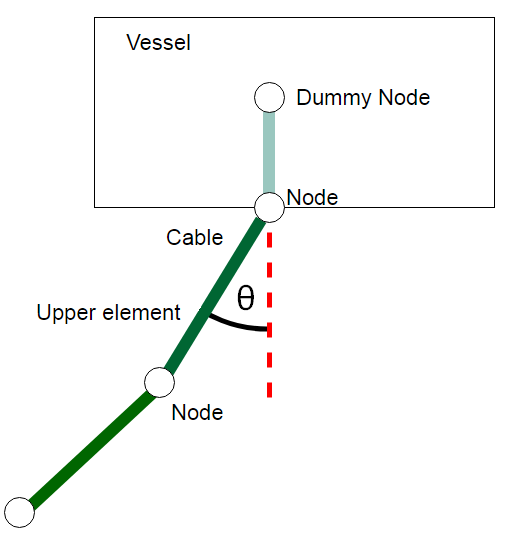
\includegraphics[scale=0.5]{figures/angle}
\caption[Angle between vessel and cable ]{Angle between vessel and cable  }
 \label{fig:angle}
\end{figure}

\begin{figure}[H]
\subfloat[Time series for angle between vessel and cable \label{fig:angleex}]
  {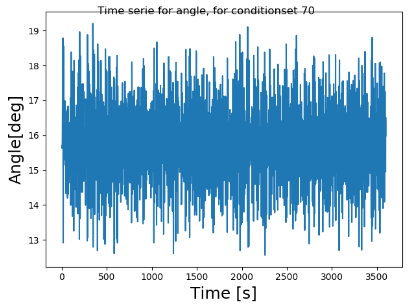
\includegraphics[width=.45\linewidth]{figures/angleex}}\hfill
\subfloat[Time series for tension in the upper element \label{fig:tensex}]
  {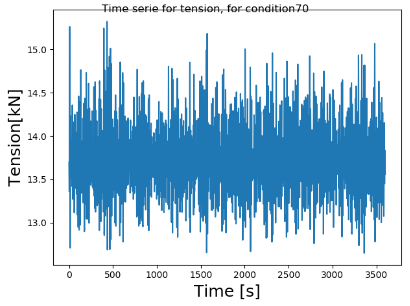
\includegraphics[width=.45\linewidth]{figures/tensex}}\hfill
\caption{Example of time series for angle and tension}
\label{fig:timeex}
\end{figure}

section{Rainflow Counting}
 Rainflow Counting was performed in Python on the time series of the angle to determine the number of cycles for each angle range. The Rainflow Counting algorithm used by Python is explained in Section \ref{sec:rainflow}. The counts from each sea state were scaled for their occurrence in the scatter diagram in Figure \ref{fig:scatn} to apply for one year according to:

\begin{equation}
    n_{cycle,year}=n_{cycle,hour} \frac{n_{seastate}}{N_{seastate}} \cdot 365 \cdot 24 
\end{equation}

\noindent Where $n_{cycle,year}$ is the number of cycles of in an angle class in a whole year, $n_{cycle,hour}$ is the number of cycles in an angle class for an hour, calculated by the global analyses, $n_{seastate}$ is the number of observations of an individual sea state according to the scatter diagram, and $N_{seastate}$ is the total number of sea states in the scatter diagram in Figure \ref{fig:scatn}.\newline
\newline 
\noindent The results from the Rainflow Counting can be seen in Figure \ref{fig:initialcyc}. The angle range classes were of equal length of 0.3, but it is not possible to see the classes on the x-axis due to a large number of classes.

\begin{figure}[H]
\centering
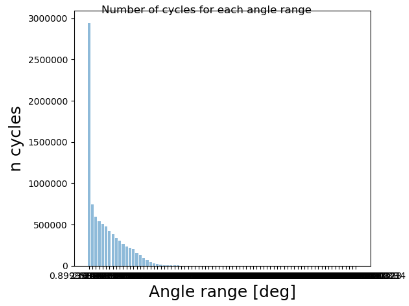
\includegraphics[scale=0.9]{figures/initialcyc}
\caption[Number of cycles in each class]{Number of cycles in each class}
 \label{fig:initialcyc}
\end{figure}

\noindent It is apparent from Figure \ref{fig:initialcyc} that the majority of the cycles are occurring in the first angle range classes, and decreasing as the angle range increases.\newline
\newline
The damage from each range was calculated according to Miner-Palmgren summation concept in Equation \ref{eq:MP}, with $N_i$ calculated from the SN-curve from Equation \ref{eq:sn}. The damage inflicted by each angle range class was calculated as:
\begin{equation}
    d_i  = \frac{n_i}{N_i}
\end{equation}
\begin{equation}
    d_i=\frac{n_i}{\frac{c}{\Delta \sigma ^m}}
\end{equation}
Where $d_i$ is the damage from the cycles in angel class i, $n_i$ is the number of cycles in angle class i, $N_i$ is the number of cycles until failure for angle class i, c and m are from Equation \ref{eq:sn}, c=4 and m=2.88e25 for this case,  $\Delta \sigma$ is the stress range that relates to the angle range as: $\Delta \sigma_i = a \Delta \theta_i$ where a is an arbitrary constant.\newline
\newline 

Figure \ref{fig:initialdam} demonstrates the damage from each angle range class. The middle classes evidently cause the most substantial damage, combining a high number of cycles with high damage per cycle. 
\begin{figure}[H]
\centering
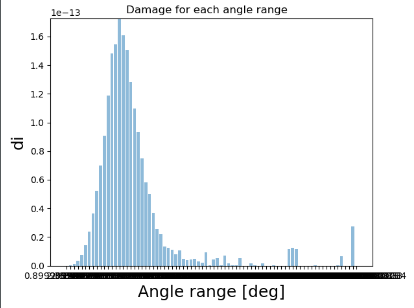
\includegraphics[scale=0.9]{figures/initialdam}
\caption[Damage for each angle class]{Damage for each angle class}
 \label{fig:initialdam}
\end{figure}
To obtain a high resolution of the final results, the angle range classes were rearranged and merged into 15 classes with approximately the same damage impact. Figure \ref{fig:initialdam} shows the damage caused by 15 rearranged angle range classes, and Figure \ref{fig:newcyc} and Table \ref{table:angleclass} present the rearranged cycle distribution.  

\begin{figure}[H]
\centering
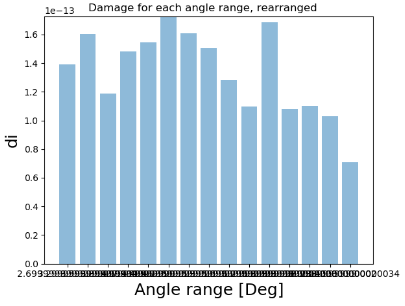
\includegraphics[scale=0.9]{figures/newdam}
\caption[Damage for each angle class, rearranged]{Damage for each angle class, rearranged}
 \label{fig:newdam}
\end{figure}

\begin{figure}[H]
\centering
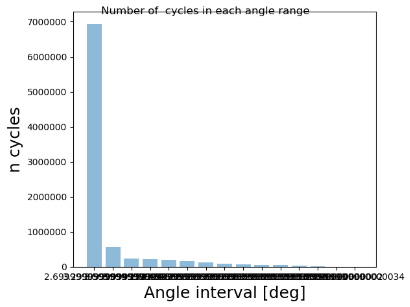
\includegraphics[scale=1]{figures/newcyc}
\caption[Distribution of cycles for each angle class, rearranged for equal damage]{Distribution of cycles for each angle class, rearranged for equal damage}
 \label{fig:newcyc}
\end{figure}

\begin{table} [H]
\centering
\begin{tabular}{ |c|c|}
\hline
Angle range class [deg] & Number of cycles \\
 \hline
 \hline
0.0 - 2.7 & 6930399.8\\

2.8 - 3.3 & 571967.9\\
 
3.4 - 3.6 & 237278.5 \\
 
3.7 - 3.9& 219492.0  \\

4.0 - 4.2& 198970.4  \\

4.3  - 4.5 & 154052.1  \\

4.6 - 4.8 & 130555.0 \\

4.9 - 5.1 & 93955.7 \\

5.2 - 5.4 & 68946.3 \\

5.5 - 5.7 & 46839.2 \\

5.8 - 6.3 & 54651.8 \\

6.4 - 6.9 & 24288.7 \\

7.0 - 8.4 & 16385.8 \\

8.5 - 18.0 & 3355.4 \\

18.1 - 23.4 & 139.3  \\

 \hline
\end{tabular}
\caption{Number of cycles in each angle range}
\label{table:angleclass}
\end{table} 
It is important to note that the cycle counts in Table \ref{table:angleclass} are not just half and whole cycles, as they were already scaled for occurrence in one year.

\section{Local Analysis}
The results from the global analyses served as input for the local analyses. Due to the nature of the boundary conditions of the local model, both ends of the model experienced rotation when a dynamic angle was applied. This is shown in Figures \ref{fig:anglecorr} and \ref{fig:anglecorrre}, where $\theta_1$ was equal to the applied angle, but the total angle experienced by the model was: 
\begin{equation}
    \theta_{tot}=\theta_1 + \theta_2
\end{equation}
Where $\theta_{tot}$ is the total angle experienced by the local model and $\theta_1$ and $\theta_2$ are illustrated in Figure \ref{fig:anglecorr}, and shown in the real model in Figure \ref{fig:anglecorrre}.

\begin{figure}[H]
\centering
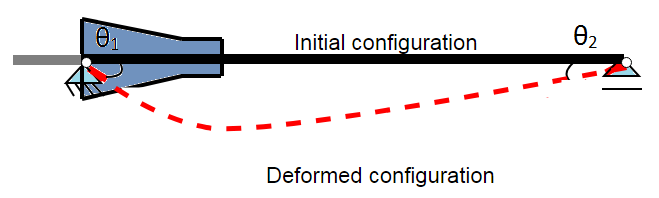
\includegraphics[scale=0.75]{figures/anglecorr1}
\caption[Initial and deformed configuration of local model]{Illustration of initial and deformed configuration of local model}
 \label{fig:anglecorr1}
\end{figure}

\begin{figure}[H]
\centering

\includegraphics[scale=0.75]{figures/anglecorrre}
\caption[Deformed local model in XPOST]{Deformed local model in XPOST}
 \label{fig:anglecorrre}
\end{figure}
 Several analyses were done to establish the relation between the applied angle and the total angle. Figure \ref{fig:anglerel} show the linear regression with a coefficient of determination ($R^2$) of 0.9978, and the relationship:
\begin{equation}
    \theta_{tot}=1.2694\theta_{appl.}
\label{eq:lincorr}
\end{equation}
Where $\theta_{tot}$ is the total angle experienced by the local model and $\theta_{appl.}$ is the angle applied by BFLEX.
\begin{figure}[H]
\centering
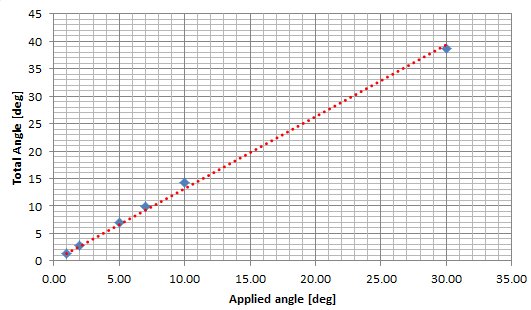
\includegraphics[scale=0.8]{figures/anglerel}
\caption[Relationship between applied angle and total angle]{Relationship between applied angle and total angle}
 \label{fig:anglerel}
\end{figure}

To determine the input the local analysis, it was decided in line with Professor Svein Sævik's recommendations that the angle would be the master over the tension. Although the trends in the angle time series and the tension time series agreed, the high angles and tensions did not occur at the exact same time steps, resulting in no linear correlation. A simple but conservative approach, with the assumption that maximum tension occurred with maximum angle, and minimum tension occurred with minimum angle, was adopted. The maximum and minimum tension recorded at the top of the cable was 40.69 kN and 9.32 kN, respectively, and linear interpolation was used to calculate the dynamic tension levels corresponding to the dynamic angle ranges in Table \ref{table:cyclecount}. \\\\Bend stiffeners are usually mounted in a stress-free configuration, equivalent to the neutral vessel position in this study. The stress-free configuration angle was -2.32$^\circ$ found from the SIMA RIFLEX, with zero degrees being as if the cable was hanging straight down and positive angle is counterclockwise. The dynamic analyses were performed in the far position with current, where the static position of the bend stiffener was 15.78$^\circ$ due to the strong current as can be seen in Figure \ref{fig:statconc}. The total mean angle was, consequently, 18.16$^\circ$, and the max and min angle for each angle range were added and subtracted to the mean angle, so that the cable oscillated about this angle.\\\\
Table  \ref{table:loadcase} display the 15 load cases for the local analysis. The angles displayed in the table are the corrected angles, calculated by Equation \ref{eq:lincorr}. The dynamic tensions were found through interpolation, and the mean tension represents the static tension at the top of the cable after the current was applied in far position. The analyses were administered by a Cygwin script, making it easy to change the variables in each case. 
\begin{table} [H]
\centering
\begin{tabular}{ |c|c|c|c|c|c|}
\hline
    Case Nr. & Max Angle [deg] & Min angle [deg] & Mean tens.[kN] & Max tens.[kN]  & Min tens.[kN]   \\
 \hline
 \hline
    1 & 16.43 & 12.18 & 13.7 & 25.07 & 11.50   \\ 
    2 &  16.91 & 11.71 & 13.7 & 25.52 & 11.44   \\
    3 &  17.14 & 11.47 & 13.7 & 25.75 & 11.41   \\ 
    4 &  17.38 & 11.23 & 13.7 & 25.97 & 11.37  \\ 
    5 &  17.61 & 11.00 & 13.7 & 26.20 & 11.34  \\ 
    6 &  17.85 & 10.76 & 13.7 & 26.42 & 11.31  \\ 
    7 &  18.09 & 10.52 & 13.7 & 26.65 & 11.28   \\ 
    8 &  18.32 & 10.29 & 13.7 & 26.88 & 11.25  \\ 
    9 &  18.56 & 10.05 & 13.7 & 27.10 & 11.22  \\ 
    10 &  18.80 & 9.82 & 13.7 & 27.33 & 11.18  \\ 
    11 & 19.27 & 9.34 & 13.7 & 27.78 & 11.12  \\ 
    12 &  19.74 & 8.87 & 13.7 & 28.24 & 11.06  \\ 
    13 &  20.92 & 7.69 & 13.7 & 29.37 & 10.90  \\ 
    14 &  28.49 & 0.13 & 13.7 & 36.62 & 9.89  \\ 
    15 &  32.74 & -4.13 & 13.7 & 40.69 & 9.32 \\ 
 \hline
\end{tabular}
\caption{Parameters for load cases in the Local Analyses}
\label{table:loadcase}
\end{table} 

\section{Calculation of Fatigue Life}
\label{sec:fatiguelife}
 The fatigue life was calculated for each layer at two points of the conductors: 
\begin{itemize}
\item At max curvature range (x=0.900m)
\item At max tension range  (x=0.625m)
\end{itemize}
The two points did not coincide due to a phase shift caused by friction. The calculation methodology was the same for both points.  \\\\ Tension and curvature plots served as outputs from the local analyses, and can be viewed in whole in Appendix \ref{appendix:C}. The output was used to calculate the stress range on wire level for each layer in each case according to the analytical model described in Section \ref{sec:fatcop}. Lay angles were $\alpha_2=-4.1^\circ$ and $\alpha_3=+7.3^\circ$ for the innermost layer and outer layer respectively,\cite{Nasution2013}. The friction coefficient was  $\mu=0.2$, and the stress concentration factor (SCF) for the innermost layer and the outer layer were 1.058 and 1.238 respectively, \cite{NASUTION2014}.\\\\
The number of cycles until failure ($N_i$) was calculated from Equation \ref{eq:sn}. Damage from each case in one year was calculated according to the Miner-Palmgren summation concept from Equation \ref{eq:MP}, using the cycle counts ($n_i$) found by Rainflow counting in Table \ref{table:angleclass}. By inverting the damage generated in one year, the fatigue life in years was calculated with a DFF=10.0. The results were mean stress corrected according to the Söderberg assumption described in Section \ref{sec:meanstress}. 

\section{Sensitivity Studies and Study of Friction Mechanisms}
Several additional studies were performed to obtain insights into the contact mechanisms in the cable cross-section. By further examination of the results collected from the global and local analyses, the following aspects were investigated:
\begin{itemize}
    \item Study of sensitivity by using mean and minimum tension in Equation \ref{eq:stressvariation2}
    \item Study of the effect of contact between conductors on fatigue life
    \item Study of the effect of contact between layers in conductors on fatigue life
\end{itemize}
All studies above were performed at the point on the conductor with maximum tension range.
\subsection{Study of Sensitivity by using Mean and Minimum Tension in Equation \ref{eq:stressvariation2}}
\label{sec:min}
Equation \ref{eq:stressvariation2}  in the analytical model does not contain specifications on which tension (T) to be used, but maximum tension yields the most conservative approach.  As a sensitivity study, the fatigue life was also calculated using the mean and minimum tension in Equation \ref{eq:stressvariation2} to see what effect this would have on the fatigue life. 
\subsection{Study of Effect of Contact Between Conductors}
The HCONT454 describes the contact between the three helical conductors in the cable cross-section. Including the contact mechanism between the conductors was investigated by looking at the plot of tension at the maximum and minimum angle in each case. Figure {fig:condfric} show the contribution to the tension range from the contact between the conductors. It was represented as the difference between the max tension range($\Delta T_{max}$) illustrated by the green arrow, and the tension range from applied tension ($\Delta T_T$) at the end of the model, illustrated by the yellow arrow.

\begin{figure}[H]
\centering
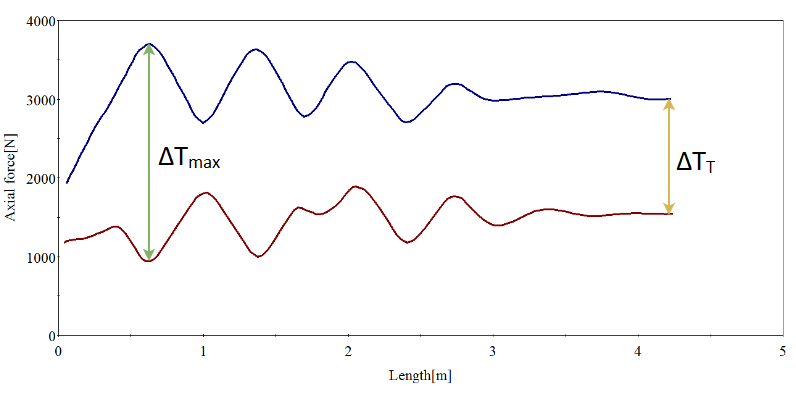
\includegraphics[scale=0.7]{figures/confric.PNG}
\caption[$\; \:$ $\Delta T_f$]{$\Delta T_f$}
 \label{fig:condfric}
\end{figure}
The contribution to the tension range from the contact friction could be calculated as:
\begin{equation}
    \Delta T_f = \Delta T_{max} - \Delta T_T
\end{equation}
Where $\sigma T_f$ is the contribution to the tension range form contact between the conductors, $\Delta T_{max}$ is the maximum tension range and $\Delta T_T$ is the tension range from applied tension to the local model. \\\\The fatigue life was calculated again with the analytical model with $\Delta T_T$ for the tension range in Equation \ref{eq:sigmaT}.

\subsection{Study of Effect of Contact Between Layers in Conductors}
The friction between the layers in the conductor was included in the analytical model by friction term, $\Delta \sigma_f^i$ in Equation \ref{eq:stressvariationred}. By eliminating this term, contact between the layers in the conductor was excluded, and  Equation \ref{eq:stressvariationred} for the stress range was reduced to:
\begin{equation}
    \Delta \sigma=\Delta \sigma_T \cdot SCF + \Delta \sigma_{nc}
\end{equation}
Calculation of fatigue life was otherwise completed according to the analytical model.




